\chapter{HOWTOs}
\label{cha:howtos}
\begin{quote}
Computers are good at following instructions, but not at reading your mind. --- Donald E. Knuth
\end{quote}
\section{Basic Tasks}
\label{sec:howto-basic-operations}
\index{how do I!basic tasks}

\subsection{How do I load a pedigree from a file?}
\label{sec:howto-load-pedigree}
\index{how do I!basic tasks!load a pedigree}
Each pedigree that you read must be passed its own dictionary of options that must have at least a pedigree file name (\var{pedfile}) and a pedigree format string (\var{pedformat}).  You then call \method{pyp_newclasses.NewPedigree()} and pass the options dictionary as an argument.  The following code fragment demonstrates how to read a pedigree file:
\begin{verbatim}
options = {}
options['pedfile'] = 'new_lacy.ped'
options['pedformat'] = 'asd'
example1 = pyp_newclasses.loadPedigree(options)
\end{verbatim}
The options dictionary may be named anything you like.  In this manual, and in the example programs distributed with \PyPedal{}, \var{options} is the name used.

\subsection{How do I load multiple pedigrees in one program?}
\label{sec:howto-load-multiple-pedigrees}
\index{how do I!basic tasks!load multiple pedigrees}
A \PyPedal{} program can load more than one pedigree at a time.  Each pedigree must be passed its own options dictionary, and the pedigrees must have different names.  This is easily done by creating a dictionary with global options and customizing it for each pedigree.  Once you have created a pedigree by calling \method{pyp\_newclasses.NewPedigree('options')} you can change the options dictionary without affecting that pedigree (a pedigree stores a copy of the options dictionary in its \member{kw} attribute).  The following code fragment demonstrates how to read two pedigree files in a single program:
\begin{verbatim}
#   Create the empty options dictionary
options = {}

#   Read the first pedigree
options['pedfile'] = 'new_lacy.ped'
options['pedformat'] = 'asd'
options['pedname'] = 'Lacy Pedigree'
example1 = pyp_newclasses.loadPedigree(options)

#   Read the second pedigree
options['pedfile'] = 'new_boichard.ped'
options['pedformat'] = 'asdg'
options['pedname'] = 'Boichard Pedigree'
example2 = pyp_newclasses.loadPedigree(options)
\end{verbatim}
Note that \var{pedformat} only needs to be changed if the two pedigrees have different formats.  You do not even have to change \var{pedfile}.

\subsection{How do I renumber a pedigree?}
\label{sec:howto-renumber-pedigree}
\index{how do I!basic tasks!renumber a pedigree}
Set the \member{renumber} option to \samp{1} before you load the pedigree.
\begin{verbatim}
options = {}
options['renumber'] = 1
options['pedfile'] = 'new_lacy.ped'
options['pedformat'] = 'asd'
example1 = pyp_newclasses.loadPedigree(options)
\end{verbatim}
If you do not renumber a pedigree at load time and choose to renumber it later you must set the \member{renumber} option and call the pedigree's \method{renumber()} method:
\begin{verbatim}
example.kw['renumber'] = 1
example.renumber()
\end{verbatim}
For more details on pedigree renumbering see Section \ref{sec:renumbering}.

\subsection{How do I turn off output messages?}
\label{sec:howto-turn-off-messages}
\index{how do I!basic tasks!turn off output}
You may want to suppress the output that is normally written to STDOUT by scripts.  You do this by setting the \member{messages} option:
\begin{verbatim}
options['messages'] = 'quiet'
\end{verbatim}
The default setting for \member{messages} is \samp{verbose}, which produces lots of messages.

\subsection{How do I load a pedigree whose columns are comma-delimited?}
\label{sec:howto-load-comma-delimited-pedigree}
\index{how do I!basic tasks!load comma-delimited pedigree}
The default column-delimiter used by \PyPedal{} is a space (` ').  Comma-separated value (CSV) files can be read by
setting \var{sepchar} to \code{','}.  If you are using a configuration file, you \emph{must} enclose the comma in
double quotation marks (``''):
\begin{verbatim}
options['sepchar'] = ","
\end{verbatim}
If you do not enclose the delimiter properly you will receive an error message such as:
\begin{verbatim}
Traceback (most recent call last):
  File "ncsu.py", line 6, in <module>
    ncsu = pyp_newclasses.loadPedigree(optionsfile='ncsu.ini', debugLoad=True)
  File "/home/jcole/sage-4.8/local/lib/python2.6/site-packages/PyPedal-2.0.3-py2.6.egg/PyPedal/pyp_newclasses.py", line 2875, in loadPedigree
    _pedigree.load(pedsource=pedsource,pedgraph=pedgraph,pedstream=pedstream)
  File "/home/jcole/sage-4.8/local/lib/python2.6/site-packages/PyPedal-2.0.3-py2.6.egg/PyPedal/pyp_newclasses.py", line 444, in load
    self.preprocess()
  File "/home/jcole/sage-4.8/local/lib/python2.6/site-packages/PyPedal-2.0.3-py2.6.egg/PyPedal/pyp_newclasses.py", line 1076, in preprocess
    l = string.split(string.strip(line),self.kw['sepchar'])
  File "/home/jcole/sage-4.8/local/lib/python2.6/string.py", line 292, in split
    return s.split(sep, maxsplit)
TypeError: expected a character buffer object
\end{verbatim}

\subsection{How do I load a pedigree whose columns are tab-delimited?}
\label{sec:howto-load-tab-delimited-pedigree}
\index{how do I!basic tasks!load tab-delimited pedigree}
The default column-delimiter used by \PyPedal{} is a space (` ').  You can change the delimiter by setting the \var{sepchar} option:
\begin{verbatim}
options['sepchar'] = '\t'
\end{verbatim}
If you are using a configuration file, you \emph{must} enclose any delimiter containing a backslash in double quotation marks (``'').
If you do not enclose the delimiter properly you will receive an error message such as:
\begin{verbatim}
[jcole@jcole2 examples]$ python new_ids.py
[INFO]: Logfile new_ids2.log instantiated.
[INFO]: Preprocessing new_ids2.ped
[INFO]: Opening pedigree file
[ERROR]: The record on line 2 of file new_ids2.ped does not have the same number
         of columns (1) as the pedigree format string (ASD) says that it should
         (3). Please check your pedigree file and the pedigree format string for
         errors.
[jcole@jcole2 examples]$
\end{verbatim}

\section{Calculating Measures of Genetic Variation}
\label{sec:howto-genetic-variation}
\index{how do I!calculate genetic variation}

\subsection{How do I calculate coefficients of inbreeding?}
\label{sec:howto-calculate-inbreeding}
\index{how do I!calculate genetic variation!coefficients of inbreeding}
This requires that you have a renumbered pedigree (HOWTO \ref{sec:howto-renumber-pedigree}).
\begin{verbatim}
options = {}
options['renumber'] = 1
options['pedfile'] = 'new_lacy.ped'
options['pedformat'] = 'asd'
example1 = pyp_newclasses.loadPedigree(options)
example_inbreeding = pyp_nrm.inbreeding(example)
print example_inbreeding
\end{verbatim}
The dictionary returned by \function{pyp_nrm.inbreeding(example)}, \var{example_inbreeding}, contains two dictionaries: \var{fx} contains coefficients of inbreeding (COI) keyed to renumbered animal IDs and \var{metadata} contains summary statistics.  \var{metadata} also contains two dictionaries: \var{all} contains summary statistics for all animals, while \var{nonzero} contains summary statistics for only animals with non-zero coefficients of inbreeding.  If you print \var{example_inbreeding} you'll get the following:
\begin{verbatim}
{'fx': {1: 0.0, 2: 0.0, 3: 0.0, 4: 0.0, 5: 0.0, 6: 0.0, 7: 0.0, 8: 0.0, 9: 0.0,
10: 0.0, 11: 0.0, 12: 0.0, 13: 0.0, 14: 0.0, 15: 0.0, 16: 0.0, 17: 0.0, 18: 0.0,
19: 0.0, 20: 0.0, 21: 0.0, 22: 0.0, 23: 0.0, 24: 0.0, 25: 0.0, 26: 0.0, 27: 0.0,
28: 0.25, 29: 0.0, 30: 0.0, 31: 0.25, 32: 0.0, 33: 0.0, 34: 0.0, 35: 0.0, 36: 0.0,
37: 0.0, 38: 0.21875, 39: 0.0, 40: 0.0625, 41: 0.0, 42: 0.0, 43: 0.03125, 44: 0.0,
45: 0.0, 46: 0.0, 47: 0.0},
'metadata': {'nonzero': {'f_max': 0.25, 'f_avg': 0.16250000000000001,
'f_rng': 0.21875, 'f_sum': 0.8125, 'f_min': 0.03125, 'f_count': 5},
'all': {'f_max': 0.25, 'f_avg': 0.017287234042553192, 'f_rng': 0.25,
'f_sum': 0.8125, 'f_min': 0.0, 'f_count': 47}}}
\end{verbatim}
Obtaining the COI for a given animal, say 28, is simple:
\begin{verbatim}
>>> print example_inbreeding['fx'][28]
'0.25'
\end{verbatim}
To print the mean COI for the pedigree:
\begin{verbatim}
>>> print example_inbreeding['metadata']['all']['f_avg']
'0.017287234042553192'
\end{verbatim}
\section{Databases and Report Generation}
\label{sec:howto-databases-and-reports}
\index{how do I!databases and reports}
\subsection{How do I load a pedigree into a database?}
\label{sec:howto-load-pedigree-db}
\index{how do I!databases and reports!load a pedigree}
The \module{pyp\_reports} module (\ref{sec:pyp-reports}) uses the \module{pyp\_db} module (Section \ref{sec:pyp-db})
to store and manipulate a pedigree in an SQLite database.  In order to use these tools you must first load your pedigree into
the database.  This is done with a call to \function{pyp\_db.loadPedigreeTable()}:
\begin{verbatim}
options = {}
options['pedfile'] = 'hartlandclark.ped'
options['pedname'] = 'Pedigree from van Noordwijck and Scharloo (1981)'
options['pedformat'] = 'asdb'

example = pyp_newclasses.loadPedigree(options)

pyp_nrm.inbreeding(example)
pyp_db.loadPedigreeTable(example)
\end{verbatim}
The routines in \module{pyp\_reports} will check to see if your pedigree has already been loaded; if it
has not, a table will be created and populated for you.
\subsection{How do I update a pedigree in the database?}
\label{sec:howto-pedigree-db-update-table}
\index{how do I!databases and reports!update pedigree table}
Changes to a \PyPedal{} pedigree object are not automatically saved to the database.  If you have changed
your pedigree, such as by calculating coefficients of inbreeding, and you want those changes visible to the
database you have to call \function{pyp\_db.loadPedigreeTable()} again.  \textbf{IMPORTANT NOTE:} If you call
\function{pyp\_db.loadPedigreeTable()} after you have already loaded your pedigree into the database it will
drop the existing table and reload it; all data in the existing table will be lost!  In the following
example, the pedigree is written to table \textbf{hartlandclark} in the database \textbf{pypedal}:
\begin{verbatim}
options = {}
options['pedfile'] = 'hartlandclark.ped'
options['pedname'] = 'Pedigree from van Noordwijck and Scharloo (1981)'
options['pedformat'] = 'asdb'

example = pyp_newclasses.loadPedigree(options)

pyp_db.loadPedigreeTable(example)
\end{verbatim}
\member{pypedal} is the default database name used by \PyPedal{}, and can be changed using a pedigree's \member{database_name} option.  By default, table names are formed from the pedigree file name.  A table name can be specified using a pedigree's \member{dbtable_name} option.  Continuing the above example, suppose that I calculated coefficients of inbreeding on my pedigree and want to store the resulting pedigree in a new table named \var{noordwijck_and_scharloo_inbreeding}:
\begin{verbatim}
options['dbtable_name'] = 'noordwijck_and_scharloo_inbreeding'
pyp_nrm.inbreeding(example)
pyp_db.loadPedigreeTable(example)
\end{verbatim}
You should see messages in the log telling you that the table has been created and populated:
\begin{verbatim}
Tue, 29 Nov 2005 11:24:22 WARNING  Table noordwijck_and_scharloo_inbreeding does
                                   not exist in database pypedal!
Tue, 29 Nov 2005 11:24:22 INFO     Table noordwijck_and_scharloo_inbreeding
                                   created in database pypedal!
\end{verbatim}
\section{Pedigrees as Graphs}
\label{sec:howto-pedigrees-graphs}
\index{how do I!pedigrees as graphs}
\PyPedal{} includes tools for working with pedigrees as algebraic structures known as directed graphs, or digraphs. Digraphs are not graphs in the sense of graphics for presentation or display. Rather, they are mathematical abstractions, the study of which can provide interesting information about the structure of a population. A digraph represents a pedigree as a set of vertices (also called nodes), which correspond to animals, and a collection of edges, which connect nodes to one another. In the context of a pedigree, edges indicate that a parent--offspring relationship exists between two animals.  If a path can be constructed between two vertices (animals) in the graph then those animals are related. If no path can be constructed between teo nodes, then no relatinship exists between the two. Routines for working with graphs (also called networwks) are contained in the \module{pyp\_network} module (\ref{sec:pyp-network})
\subsection{How do I convert a pedigree to a graph?}
\label{sec:howto-pedigree-to-graph}
\index{how do I!pedigrees as graphs!pedigree to graph}
The function \function{pyp\_network.ped\_to\_graph()} takes a \PyPedal{} pedigree object as its argument and returns a NetworkX (\url{https://networkx.lanl.gov/}) XDiGraph object:
\begin{verbatim}
example = pyp_newclasses.loadPedigree(optionsfile='new_networkx.ini')
ng = pyp_network.ped_to_graph(example)
\end{verbatim}
Once you've got a graph, you use the NetworkX API to operate on the graph. For example, the number of animals in the pedigree is simply the number of nodes in the graph:
\begin{verbatim}
print 'Number of animals in pedigree: %s' % ( ng.order() )
print ng.nodes()
\end{verbatim}
\subsection{How do I convert a graph to a pedigree?}
\label{sec:howto-graph-to-pedigree}
\index{how do I!pedigrees as graphs!graph to pedigree}
It is possible to create a \PyPedal{} pedigree from a NetworkX graph. This is useful, for example, when you'd like to create a pedigree representing a subset of the population in a \class{NewPedigree} object. \function{pyp\_nrm.recurse\_pedigree()} and related functions won't do the trick because they return only lists of animal IDs, not actual \class{NewPedigree} instances. To create a pedigree from a graph you simply build your options dictionary and call \function{pyp\_newclasses.loadPedigree()}:
\begin{verbatim}
options = {}
options['pedfile'] = 'dummy'
options['messages'] = 'verbose'
options['renumber'] = 1
options['pedname'] = 'Testing fromgraph()'
options['pedformat'] = 'asd'
options['set_offspring'] = 1
options['set_ancestors'] = 1
options['set_sexes'] = 1
options['set_generations'] = 1
example2 = pyp_newclasses.loadPedigree(options,pedsource='graph',pedgraph=ng)
\end{verbatim}
You must provide a non-null \texttt{pedfile} keyword in your options dictionary, as well as the \texttt{pedsource} and \texttt{pedgraph} arguments to \function{pyp\_newclasses.loadPedigree()}.

There is a known bug with logfile creation when loading a pedigree from a digraph.
\subsection{How do I load a pedigree from a file containing a graph stored as an adjacency list?}
\label{sec:howto-pedigree-from-graph-file}
\index{how do I!pedigrees as graphs!pedigree from graph file}
\PyPedal{} can read graphs stored in text files as adjacency lists, which is one way of representing directed graphs:
\begin{verbatim}
options = {}
options['pedfile'] = 'pedigree.adjlist'
options['messages'] = 'verbose'
options['pedname'] = 'Testing graphfile'
options['pedformat'] = 'asd'
example = pyp_newclasses.loadPedigree(options,pedsource='graphfile')
\end{verbatim}
\subsection{How do I save a graph as an adjacency list?}
\label{sec:howto-graph-to-file}
\index{how do I!pedigrees as graphs!graph to file}
\PyPedal{}, using NetworkX, can save graphs as adjacency lists:
\begin{verbatim}
example.savegraph('pedigree.adjlist')
\end{verbatim}
\section{Miscellaneous}
\label{sec:howto-miscellaneous}
\index{how do I!miscellaneous}
\subsection{How do I export a numerator relationship matrix so that I can read it into Octave?}
\label{sec:howto-export-nrm-to-octave}
\index{how do I!miscellaneous!export NRM to Octave}
Numerator relationship matrices may be exported to text files for use with, e.g., Octave using the \method{NewAMatrix.save} method:
\begin{verbatim}
example = pyp_newclasses.loadPedigree(optionsfile='denny.ini')
amatrix = pyp_newclasses.NewAMatrix(example.kw)
amatrix.form_a_matrix(example.pedigree)
amatrix.tofile('Ainv.txt')
\end{verbatim}
When matrices are written to text files array elements are separated by \var{sepchar} (Table \ref{tbl:options}).

Matrices may also be written to a binary format. The default value of the \var{nrm\_format} pedigree option is \texttt{text}. To write files in binary format you must either specify the  value of the \var{nrm\_format} option as \texttt{binary} before you load your pedigree file or use the \var{nrm\_format} keyword when you call \method{NewAMatrix.save}:
\begin{verbatim}
amatrix.tofile('Ainv.bin',nrm_format='binary')
\end{verbatim}
Once you've saved the NRM to a file, say \texttt{'Ainv.txt'}, in text format you can easily read it into Octave:
\begin{verbatim}
octave:1> myfile = fopen ("Ainv.txt", "r");
octave:2> ainv = fscanf(myfile,'%f',[18,18])
\end{verbatim}
This has been verified with Octave 2.1.57 under RedHat Enterprise Linux on small matrices.
\subsection{How else can I export a NRM to a file?}
\label{sec:howto-export-nrm-to-ijk-file}
\index{how do I!miscellaneous!export NRM to a file}
Numerator relationship matrices may be exported to a text file in ``ijk format'',
where each line is of the form ``animal\_A animal\_B rAB'' using the \function{pyp\_io.save\_ijk()} function. Diagonal entries are $1 + f_a$, where $f_a$ is the animal's coefficient of inbreedin.
\begin{verbatim}
example = pyp_newclasses.loadPedigree(options)
# Save the NRM to a file in ijk format.
# Don't forget to set the filename.
pyp_io.save_ijk(example,'nrm_ijk.txt')
\end{verbatim}
Suppose that the example above produces the following file:
\begin{verbatim}
$ head nrm_ijk.txt
4627 4627 1.125
4627 0832 0.0
4627 5538 0.5
...
\end{verbatim}
In order to get $f_a$ for animal 4627 you need to find the corresponding diagonal element and subtract 1 from it:
\[
f_a = 1.125 - 1.0 = 0.125
\]
The coefficient of relationship between 4627 and 5538 is $0.5$ (4627 is probably a parent of 5538). Note that the file \var{nrm\_ijk.txt} will include only the diagonal and upper off-diagonal elements of the NRM, and should have $n + n(n+1)/2$ lines.
\subsection{How do I load a pedigree from a GEDCOM file?}
\label{sec:howto-load-gedcom-pedigree}
\index{how do I!miscellaneous!load a GEDCOM pedigree}
As of version 2 release candidate 1 \PyPedal{} can load pedigrees from GEDCOM 5.5 files. This is done by passing the \function{pedsource}\index{pedsource} keyword to \function{pyp_newclasses.loadPedigree} with a value of \samp{gedcomfile}:
\begin{verbatim}
options['pedfile'] = 'example2.ged'
options['pedformat'] = 'ASD'
options['pedname'] = 'A GEDCOM pedigree'
example2 = pyp_newclasses.loadPedigree(options,pedsource='gedcomfile')
\end{verbatim}
Note that only a limited subset of the GEDCOM format is supported, and it is possible to lose metadata when converting a pedigree from GEDCOM to \PyPedal{}. More details on \PyPedal{}'s GEDCOM handling can be found in Appendix \ref{GEDCOM}.
\subsection{How do I save a pedigree to a GEDCOM file?}
\label{sec:howto-save-gedcom-pedigree}
\index{how do I!miscellaneous!save to GEDCOM pedigree}
As of version 2 release candidate 1 \PyPedal{} can write pedigrees to GEDCOM 5.5-formatted files using the \function{savegedcom}\index{savegedcom} method of \function{pyp_newclasses.NewPedigree} objects. The method takes an output file name as its argument:
\begin{verbatim}
 test.savegedcom('ged3.pypedal.ged')
\end{verbatim}
Note that not all attributes of \function{pyp_newclasses.NewAnimal} objects are written to the output file. More details on \PyPedal{}'s GEDCOM handling can be found in Appendix \ref{GEDCOM}.
\subsection{How do I load a pedigree from a string?}
\label{sec:howto-load-from-string}
\index{how do I!miscellaneous!load a pedigree from a string}
There are some use cases for which it is desirable to load pedigrees from strings rather than from files. This is done by passing the \function{pedsource}\index{pedsource} keyword to \function{pyp_newclasses.loadPedigree} with a value of \samp{textstream}, along with a string named \samp{pedstream} (Figure \ref{fig:ped-from-string}):
\begin{verbatim}
options = {}
options['pedfile'] = ''
options['renumber'] = 1
options['pedformat'] = 'ASD'
if __name__ == "__main__":
    pedstream = 'a1,s1,d1\na2,s2,d2\na3,a1,a2\n'
    test = pyp_newclasses.loadPedigree(options,pedsource='textstream',pedstream=pedstream)
    pyp_graphics.new_draw_pedigree(test, gfilename='partial', gtitle='Text Stream', gorient='p',gname=1)
\end{verbatim}
Note that only ASD-formatted pedigrees can be loaded this way, individual IDs are separated with commas, and successive records are separated by newlines. All records must contain a newline, including the last record in the string! You must also set the \samp{pedfile} option to a value, even if that value is just an empty string as in the example.
\begin{figure}
  \begin{center}
    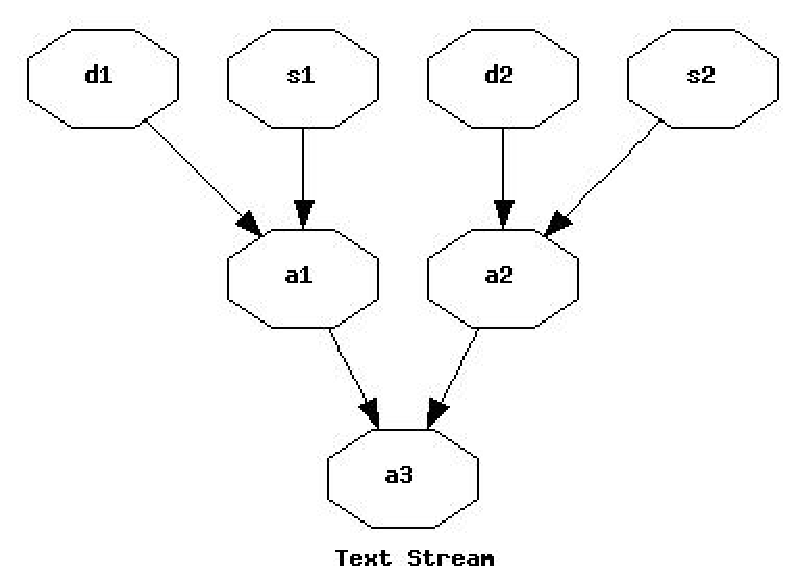
\includegraphics[width=4in]{pedfromstring.eps}
    \caption{Pedigree loaded from a string}
    \label{fig:ped-from-string}
  \end{center}
\end{figure}
\section{Contribute a HOWTO}
\label{sec:howto-contribute}
\index{how do I!contribute a HOWTO}
Users are invited to contribute HOWTOs demonstrating how to solve problems they've found interesting.  In order for such HOWTOs to be considered for inclusion in this manual they must be licensed under the GNU Free Documentation License version 1.2 or later (\url{http://www.gnu.org/copyleft/fdl.html}).  Authorship will be acknowledged, and copyright will remain with the author of the HOWTO.
